\ifdefined\inMainDoc\else
\documentclass[12pt,a4paper]{article}
% ================================================================
%  PRÉAMBULE COMMUN - ANNALES CORRIGÉES
%  Université de Kara - FaST - Licence Fondamentale MPC
%  Design optimisé impression noir et blanc
% ================================================================

% -- ENCODAGE & LANGUE --
\usepackage[utf8]{inputenc}
\usepackage[T1]{fontenc}
\usepackage[french]{babel}
\usepackage{lmodern}
\usepackage{microtype}

% -- MISE EN PAGE --
\usepackage[a4paper, top=2.8cm, bottom=2.5cm, left=2.5cm, right=2.5cm, headheight=14pt]{geometry}
\usepackage{setspace}
\setstretch{1.2}
\usepackage{parskip}
\setlength{\parindent}{1.2em}
\setlength{\parskip}{4pt}

% -- MATHS --
\usepackage{amsmath, amssymb, mathtools, amsthm}
\usepackage{mathrsfs}
\usepackage{dsfont}
\usepackage{bm}
\usepackage{cancel}
\usepackage{textcomp}
% Définition de \oiint (intégrale de surface fermée) sans package supplémentaire
\newcommand{\oiint}{\mathop{\iint\!\!\!\!\!\!\!\bigcirc}\limits}

% -- PHYSIQUE & CHIMIE --
\usepackage{physics}
\usepackage{siunitx}
% Lorsque physics est chargé, siunitx omet \qty. On le restaure ici :
\AtBeginDocument{\RenewCommandCopy\qty\SI}
\sisetup{locale = FR, detect-all, output-decimal-marker={,}}
% Commande de substitution pour les unités posant problème avec pdflatex
% (ohm, degreeCelsius, micro, angstrom, percent utilisent des caractères non-ASCII)
\newcommand{\qtyohm}[1]{\ensuremath{\num{#1}\,\Omega}}
\newcommand{\qtydegc}[1]{\ensuremath{\num{#1}\,{}^\circ\text{C}}}
\newcommand{\qtyangstrom}[1]{\ensuremath{\num{#1}\,\text{\AA}}}
\newcommand{\qtypercent}[1]{\ensuremath{\num{#1}\,\%}}
\newcommand{\qtyum}[1]{\ensuremath{\num{#1}\,\mu\text{m}}}
\usepackage[version=4]{mhchem}

% -- GRAPHISMES --
\usepackage{graphicx}
\usepackage{float}
\usepackage{caption}
\usepackage{subcaption}
\usepackage{wrapfig}
\usepackage{tikz}
\usetikzlibrary{calc, arrows.meta, patterns, shapes.geometric}
\usepackage{pgfplots}
\pgfplotsset{compat=1.18}

% -- TABLEAUX --
\usepackage{booktabs}
\usepackage{array}
\usepackage{tabularx}
\usepackage{multirow}

% -- LISTES --
\usepackage{enumitem}
\setlist[enumerate]{topsep=3pt, itemsep=2pt, parsep=0pt}
\setlist[itemize]{topsep=3pt, itemsep=2pt, parsep=0pt, label={.}}

% -- BOÎTES (noir et blanc) --
\usepackage{mdframed}
\usepackage{tcolorbox}
\tcbuselibrary{skins, breakable, theorems}

% Boîte EXERCICE : encadré avec filet épais, fond blanc
\newmdenv[
  linewidth=1.2pt,
  linecolor=black,
  roundcorner=3pt,
  skipabove=10pt,
  skipbelow=6pt,
  innertopmargin=8pt,
  innerbottommargin=8pt,
  innerleftmargin=10pt,
  innerrightmargin=10pt,
  backgroundcolor=white,
  frametitle={\bfseries\small Exercice},
  frametitlealignment=\raggedright,
  frametitleaboveskip=4pt,
  frametitlebelowskip=4pt,
]{boiteexercice}

% Boîte CORRIGÉ : fond gris très clair + filet fin
\newmdenv[
  linewidth=0.6pt,
  linecolor=black,
  leftline=true,
  rightline=false,
  topline=false,
  bottomline=false,
  linecolor=black,
  innerleftmargin=12pt,
  innerrightmargin=8pt,
  innertopmargin=6pt,
  innerbottommargin=6pt,
  backgroundcolor=gray!8,
  skipabove=4pt,
  skipbelow=8pt,
]{boitecorrige}

% Boîte RÉSUMÉ DE COURS : double encadré
\newmdenv[
  linewidth=0.8pt,
  linecolor=black,
  roundcorner=2pt,
  backgroundcolor=gray!12,
  innertopmargin=10pt,
  innerbottommargin=10pt,
  innerleftmargin=12pt,
  innerrightmargin=12pt,
  skipabove=12pt,
  skipbelow=8pt,
]{boiteresume}

% Boîte ATTENTION/REMARQUE : barre gauche épaisse
\newmdenv[
  leftline=true,
  rightline=false,
  topline=false,
  bottomline=false,
  linewidth=3pt,
  linecolor=black,
  backgroundcolor=gray!5,
  innerleftmargin=12pt,
  innerrightmargin=8pt,
  innertopmargin=5pt,
  innerbottommargin=5pt,
  skipabove=6pt,
  skipbelow=6pt,
]{boiteremarque}

% -- DIFFICULTÉ DES EXERCICES --
\newcommand{\facile}{$\star$}
\newcommand{\moyen}{$\star\!\star$}
\newcommand{\difficile}{$\star\!\star\!\star$}
\newcommand{\niveau}[1]{\hfill\textbf{#1}\hspace{2pt}}

% -- EN-TÊTES ET PIEDS DE PAGE --
\usepackage{fancyhdr}
\pagestyle{fancy}
\fancyhf{}
\renewcommand{\headrulewidth}{0.5pt}
\renewcommand{\footrulewidth}{0.3pt}

% -- HYPERLIENS --
\usepackage[hidelinks]{hyperref}
\hypersetup{
    colorlinks=false,
    pdftitle={Annale Corrigée - Licence MPC - Université de Kara}
}

% -- TITRES --
\usepackage{titlesec}
\titleformat{\section}{\Large\bfseries}{\thesection.}{0.8em}{}[\vspace{2pt}\hrule\vspace{4pt}]
\titleformat{\subsection}{\large\bfseries}{\thesubsection.}{0.7em}{}
\titleformat{\subsubsection}{\normalsize\bfseries}{\thesubsubsection.}{0.6em}{}

% -- THÉORÈMES --
\theoremstyle{definition}
\newtheorem{defn}{Définition}[section]
\newtheorem{prop}{Propriété}[section]
\newtheorem{thm}{Théorème}[section]
\newtheorem{corol}{Corollaire}[section]
\newtheorem{exemple}{Exemple}[section]

% -- COMMANDES MATHÉMATIQUES UTILES --
\newcommand{\vect}[1]{\overrightarrow{#1}}
\newcommand{\R}{\mathbb{R}}
\newcommand{\N}{\mathbb{N}}
\newcommand{\Z}{\mathbb{Z}}
\newcommand{\C}{\mathbb{C}}
\renewcommand{\d}{\mathrm{d}}
\newcommand{\deriv}[2]{\dfrac{\d #1}{\d #2}}
\newcommand{\dpart}[2]{\dfrac{\partial #1}{\partial #2}}
\newcommand{\rot}{\overrightarrow{\mathrm{rot}}\,}
\renewcommand{\div}{\mathrm{div}\,}
\renewcommand{\grad}{\overrightarrow{\mathrm{grad}}\,}
\newcommand{\e}{\mathrm{e}}
\newcommand{\ii}{\mathrm{i}}
\renewcommand{\Tr}{\mathrm{Tr}}

% Numérotation des équations par section
\numberwithin{equation}{section}

% -- RÉSULTATS ENCADRÉS --
\newcommand{\res}[1]{\[\boxed{#1}\]}

% -- REMARQUE INLINE --
\newcommand{\rmq}[1]{\begin{boiteremarque}\textbf{Remarque.} #1\end{boiteremarque}}

% -- MISE EN VALEUR DU RÉSULTAT FINAL --
\newcommand{\reponse}[1]{%
  \begin{center}
    \fbox{\begin{minipage}{0.92\textwidth}\centering #1\end{minipage}}
  \end{center}%
}


\lhead{\small\textit{Physique des Semi-conducteurs - Licence 2}}
\rhead{\small\textit{FaST, Université de Kara}}
\cfoot{\thepage}

\begin{document}
\fi

\begin{center}
  {\LARGE\bfseries PHYSIQUE DES SEMI-CONDUCTEURS}\\[0.3cm]
  {\normalsize Licence 2 - Mathématiques, Physique et Chimie}\\[0.1cm]
  \rule{0.7\textwidth}{0.8pt}
\end{center}

\section*{Résumé du cours}

\begin{boiteresume}

\textbf{1. Structure de bande.} Dans un solide cristallin, les niveaux d'énergie des électrons se regroupent en bandes. La bande de valence est la bande la plus haute entièrement remplie à 0\,K. La bande de conduction est la première bande vide. Le gap $E_g$ sépare ces deux bandes. Les \textit{conducteurs} ont $E_g=0$, les \textit{isolants} ont $E_g>4\,\text{eV}$, les \textit{semi-conducteurs} ont $E_g$ de l'ordre de 1\,eV.

\textbf{2. Semi-conducteurs intrinsèques.} À température finie, des électrons franchissent le gap par agitation thermique, laissant des trous dans la bande de valence. La densité intrinsèque : $n_i = \sqrt{n\cdot p}$ avec $np = n_i^2 = C T^3\e^{-E_g/k_BT}$.

\textbf{3. Semi-conducteurs dopés.} Dopage de type N (donneurs) : introduction d'impuretés pentavalentes (phosphore dans le silicium) ; les électrons sont majoritaires. Dopage de type P (accepteurs) : impuretés trivalentes (bore) ; les trous sont majoritaires. La loi d'action de masse : $np = n_i^2$.

\textbf{4. Statistique de Fermi-Dirac.} La probabilité d'occupation d'un état d'énergie $E$ est $f(E) = \dfrac{1}{1+\e^{(E-E_F)/k_BT}}$ où $E_F$ est le niveau de Fermi. Pour un semi-conducteur intrinsèque, $E_F$ est approximativement au milieu du gap.

\textbf{5. Transport des porteurs.} Courant de dérive : $\vec{J} = (n\mu_n + p\mu_p)e\vec{E}$ ($\mu_{n,p}$ : mobilités). Courant de diffusion : $\vec{J}_n = eD_n\nabla n$, $\vec{J}_p = -eD_p\nabla p$. Relation d'Einstein : $D = \mu k_BT/e$.

\textbf{6. Jonction p-n.} Interface entre un matériau p et un matériau n. En l'absence de polarisation, une zone de déplétion se crée avec un champ interne $E_0$ et une tension de contact $V_0$. Caractéristique I-V : $I = I_s(\e^{eV/k_BT}-1)$ (équation de Shockley).

\end{boiteresume}

\newpage
\section{Structure de bande et porteurs}

\subsection*{Exercice 1 - Semi-conducteur intrinsèque \niveau{\facile}}

\begin{boiteexercice}
Le silicium (Si) a un gap $E_g = \qty{1.12}{eV}$ à 300\,K. La densité intrinsèque de porteurs est $n_i = \qty{1.5e10}{cm^{-3}}$.
\begin{enumerate}
  \item Quelle est la densité d'électrons $n$ dans le Si intrinsèque à 300\,K ?
  \item Quelle est la densité de trous $p$ ?
  \item Si l'on dope avec $N_D = 10^{16}\,\text{cm}^{-3}$ atomes donneurs, calculer $n$ et $p$ à 300\,K (on suppose ionisation complète).
  \item Quelle est la conductivité du Si dopé sachant que $\mu_n = \qty{1350}{cm^2.V^{-1}.s^{-1}}$ et $\mu_p = \qty{480}{cm^2.V^{-1}.s^{-1}}$ ?
\end{enumerate}
\end{boiteexercice}

\begin{boitecorrige}
\textbf{1.} Dans le Si intrinsèque : $n = n_i = \qty{1.5e10}{cm^{-3}}$.

\textbf{2.} De même, $p = n_i = \qty{1.5e10}{cm^{-3}}$ (autant d'électrons que de trous créés par paire).

\textbf{3.} Avec $N_D = 10^{16}\,\text{cm}^{-3} \gg n_i$ (ionisation complète, neutralité de charge) :
\[
n \approx N_D = 10^{16}\,\text{cm}^{-3}
\]
La loi d'action de masse donne la densité de trous minoritaires :
\[
p = \frac{n_i^2}{n} = \frac{(1{,}5\times10^{10})^2}{10^{16}} = \frac{2{,}25\times10^{20}}{10^{16}} = \qty{2.25e4}{cm^{-3}}
\]

\textbf{4.} La conductivité est dominée par les porteurs majoritaires (électrons) :
\[
\sigma = e(n\mu_n + p\mu_p) \approx en\mu_n = 1{,}6\times10^{-19}\times10^{16}\times1350 = \qty{2.16}{S.cm^{-1}}
\]
(La contribution des trous $ep\mu_p = 1{,}6\times10^{-19}\times2{,}25\times10^4\times480 \approx \qty{1.7e-12}{S.cm^{-1}}$ est négligeable.)
\end{boitecorrige}

\subsection*{Exercice 2 - Niveau de Fermi \niveau{\moyen}}

\begin{boiteexercice}
Dans un semi-conducteur de type N avec $N_D = \qty{5e15}{cm^{-3}}$ à $T=300$\,K, la densité d'états effective de la bande de conduction est $N_C = \qty{2.8e19}{cm^{-3}}$.
\begin{enumerate}
  \item Rappeler l'expression de la densité d'électrons $n$ en fonction du niveau de Fermi $E_F$ et du bas de la bande de conduction $E_C$.
  \item Calculer $E_C - E_F$ (en eV).
  \item Que se passe-t-il si $N_D$ augmente ? Le niveau de Fermi se rapproche-t-il ou s'éloigne-t-il de $E_C$ ?
\end{enumerate}
\end{boiteexercice}

\begin{boitecorrige}
\textbf{1.} Dans l'approximation de Maxwell-Boltzmann (valide lorsque $E_C-E_F\gg k_BT$) :
\[
n = N_C\,\e^{-(E_C-E_F)/k_BT}
\]

\textbf{2.} Avec $n\approx N_D = 5\times10^{15}\,\text{cm}^{-3}$ :
\[
\e^{-(E_C-E_F)/k_BT} = \frac{N_D}{N_C} = \frac{5\times10^{15}}{2{,}8\times10^{19}} = 1{,}786\times10^{-4}
\]
\[
E_C - E_F = -k_BT\ln\!\left(\frac{N_D}{N_C}\right) = -0{,}02585\times\ln(1{,}786\times10^{-4})
\]
\[
= -0{,}02585\times(-8{,}63) \approx \qty{0.223}{eV}
\]
Le niveau de Fermi est à $0{,}223\,\text{eV}$ en dessous du bas de la bande de conduction.

\textbf{3.} Si $N_D$ augmente, $n$ augmente, $\e^{-(E_C-E_F)/k_BT}$ augmente, donc $E_C-E_F$ diminue : le niveau de Fermi \textbf{se rapproche} de $E_C$. À très fort dopage, $E_F$ peut entrer dans la bande de conduction (semi-conducteur dégénéré).
\end{boitecorrige}

\section{Jonction p-n}

\subsection*{Exercice 3 - Jonction p-n à l'équilibre \niveau{\moyen}}

\begin{boiteexercice}
Une jonction p-n en silicium possède $N_A = 10^{17}\,\text{cm}^{-3}$ côté p et $N_D = 10^{16}\,\text{cm}^{-3}$ côté n. À 300\,K, $n_i = \qty{1.5e10}{cm^{-3}}$ et $k_BT/e = \qty{25.85}{mV}$.
\begin{enumerate}
  \item Calculer la tension de contact $V_0 = \frac{k_BT}{e}\ln\!\left(\frac{N_A N_D}{n_i^2}\right)$.
  \item Quel est le signe de la tension de contact (côté p par rapport au côté n) ?
  \item La jonction est polarisée en direct avec $V = \qty{0.6}{V}$. Quel est le rapport $I/I_s$ ?
\end{enumerate}
\end{boiteexercice}

\begin{boitecorrige}
\textbf{1.}
\[
V_0 = 0{,}02585\times\ln\!\left(\frac{10^{17}\times10^{16}}{(1{,}5\times10^{10})^2}\right)
= 0{,}02585\times\ln\!\left(\frac{10^{33}}{2{,}25\times10^{20}}\right)
\]
\[
= 0{,}02585\times\ln(4{,}44\times10^{12}) = 0{,}02585\times29{,}12 \approx \qty{0.753}{V}
\]

\textbf{2.} La tension de contact est positive côté n par rapport au côté p. Autrement dit, le potentiel électrostatique est plus élevé côté n. Du côté p, il y a accumulation de charges négatives (accepteurs ionisés) et du côté n, de charges positives (donneurs ionisés).

\textbf{3.} Avec $V=\qty{0.6}{V}$ :
\[
I = I_s\left(\e^{V/(k_BT/e)}-1\right) \approx I_s\,\e^{0{,}6/0{,}02585} = I_s\,\e^{23{,}2}
\]
\[
\frac{I}{I_s} = \e^{23{,}2} \approx 1{,}2\times10^{10}
\]
En polarisation directe, le courant est environ $10^{10}$ fois plus grand que le courant de saturation.
\end{boitecorrige}

\subsection*{Exercice 4 - Transistor bipolaire \niveau{\difficile}}

\begin{boiteexercice}
Un transistor bipolaire NPN est en régime actif direct. Le courant de collecteur est $I_C = \qty{5}{mA}$ et le gain en courant en base commune est $\alpha = 0{,}99$.
\begin{enumerate}
  \item Calculer le courant d'émetteur $I_E$.
  \item Calculer le gain en courant en émetteur commun $\beta = \alpha/(1-\alpha)$.
  \item Calculer le courant de base $I_B$.
  \item Si la résistance de collecteur $R_C = \qty{1}{k\Omega}$ et l'alimentation $V_{CC} = \qty{12}{V}$, quelle est la tension $V_{CE}$ ?
\end{enumerate}
\end{boiteexercice}

\begin{boitecorrige}
\textbf{1.} En base commune : $I_C = \alpha I_E$, donc :
\[
I_E = \frac{I_C}{\alpha} = \frac{5}{0{,}99} \approx \qty{5.05}{mA}
\]

\textbf{2.} $\beta = \dfrac{\alpha}{1-\alpha} = \dfrac{0{,}99}{0{,}01} = 99$.

\textbf{3.} $I_B = I_E - I_C = 5{,}05 - 5 = \qty{0.05}{mA}$. Vérification : $I_C = \beta I_B = 99\times0{,}05 = \qty{4.95}{mA} \approx \qty{5}{mA}$.

\textbf{4.} La loi des mailles au collecteur ($V_{CC} = R_C I_C + V_{CE}$) :
\[
V_{CE} = V_{CC} - R_C I_C = 12 - 1000\times5\times10^{-3} = 12 - 5 = \qty{7}{V}
\]
Le transistor est bien en régime actif (pas saturé) puisque $V_{CE}>V_{CE,sat}\approx0{,}2\,\text{V}$.
\end{boitecorrige}

\section{Porteurs minoritaires et recombinaison}

\subsection*{Exercice 5 - Concentration intrinsèque et loi de masse action \niveau{\moyen}}

\begin{boiteexercice}
Le germanium (Ge) a les paramètres suivants à $T = \qty{300}{K}$ : gap $E_g = \qty{0.67}{eV}$, densités d'états effectives $N_C = \qty{1.04e19}{cm^{-3}}$ et $N_V = \qty{6.0e18}{cm^{-3}}$, constante de Boltzmann $k_B = \qty{8.617e-5}{eV.K^{-1}}$.
\begin{enumerate}
  \item Rappeler l'expression de la concentration intrinsèque $n_i$ en fonction de $N_C$, $N_V$, $E_g$ et $T$.
  \item Calculer $n_i$ pour le Ge à 300\,K.
  \item Comparer avec le Si ($n_i = \qty{1.5e10}{cm^{-3}}$). Lequel conduit mieux à température ambiante ?
  \item On dope le Ge avec $N_A = \qty{1e14}{cm^{-3}}$ accepteurs. Calculer $p$, $n$ et la résistivité si $\mu_p = \qty{1900}{cm^2.V^{-1}.s^{-1}}$ et $\mu_n = \qty{3900}{cm^2.V^{-1}.s^{-1}}$.
\end{enumerate}
\end{boiteexercice}

\begin{boitecorrige}
\textbf{1.} La concentration intrinsèque est :
\[
n_i = \sqrt{N_C N_V}\,\e^{-E_g/(2k_BT)}
\]

\textbf{2.} Application numérique pour le Ge à 300\,K ($k_BT = 0{,}02585\,\text{eV}$) :
\[
\sqrt{N_C N_V} = \sqrt{1{,}04\times10^{19}\times6{,}0\times10^{18}} = \sqrt{6{,}24\times10^{37}} \approx \qty{7.9e18}{cm^{-3}}
\]
\[
\e^{-E_g/(2k_BT)} = \e^{-0{,}67/(2\times0{,}02585)} = \e^{-12{,}96} \approx 2{,}34\times10^{-6}
\]
\[
\boxed{n_i \approx 7{,}9\times10^{18}\times2{,}34\times10^{-6} \approx \qty{1.85e13}{cm^{-3}}}
\]

\textbf{3.} Le Ge a $n_i \approx \qty{1.85e13}{cm^{-3}} \gg n_i(\text{Si}) = \qty{1.5e10}{cm^{-3}}$. Le Ge conduit mieux à température ambiante car son gap est plus petit (moins d'énergie nécessaire pour créer des porteurs).

\textbf{4.} Avec $N_A = \qty{1e14}{cm^{-3}}$ et $n_i = \qty{1.85e13}{cm^{-3}}$ (ici $N_A > n_i$) :
\[
p = \frac{N_A}{2} + \sqrt{\left(\frac{N_A}{2}\right)^2 + n_i^2} = 5\times10^{13} + \sqrt{25\times10^{26} + 3{,}42\times10^{26}} \approx \qty{1.18e14}{cm^{-3}}
\]
\[
n = \frac{n_i^2}{p} = \frac{(1{,}85\times10^{13})^2}{1{,}18\times10^{14}} \approx \qty{2.9e12}{cm^{-3}}
\]
La résistivité (dominée par les trous) :
\[
\sigma = e(p\mu_p + n\mu_n) \approx 1{,}6\times10^{-19}\times1{,}18\times10^{14}\times1900 \approx \qty{3.58e-2}{S.cm^{-1}}
\]
\[
\rho = 1/\sigma \approx \qty{27.9}{\Omega.cm}
\]
\end{boitecorrige}

\subsection*{Exercice 6 - Bandes d'énergie et classification des solides \niveau{\facile}}

\begin{boiteexercice}
On compare trois matériaux : le cuivre (Cu), le silicium (Si) et l'oxyde de silicium (SiO$_2$).
\begin{enumerate}
  \item Définir la bande de valence, la bande de conduction et le gap $E_g$.
  \item Classer ces matériaux en conducteur, semi-conducteur ou isolant :
  Cu ($E_g \approx 0$), Si ($E_g = \qty{1.12}{eV}$), SiO$_2$ ($E_g \approx \qty{9}{eV}$).
  \item Expliquer qualitativement pourquoi la résistivité d'un
  semi-conducteur \emph{diminue} lorsque la température augmente
  (comportement opposé aux métaux).
  \item Le Si intrinsèque vérifie $n_i = \qty{1.5e10}{cm^{-3}}$ à
  300\,K et la loi
  \[ n_i(T) \propto T^{3/2}\,\e^{-E_g/(2k_BT)}. \]
  Estimer le rapport $n_i(400\,\text{K})/n_i(300\,\text{K})$.
\end{enumerate}
\end{boiteexercice}

\begin{boitecorrige}
\textbf{1.} La \textbf{bande de valence} est la dernière bande entièrement remplie d'électrons à 0\,K. La \textbf{bande de conduction} est la première bande vide. Le \textbf{gap} $E_g$ est l'énergie qui sépare le haut de la bande de valence du bas de la bande de conduction.

\begin{center}
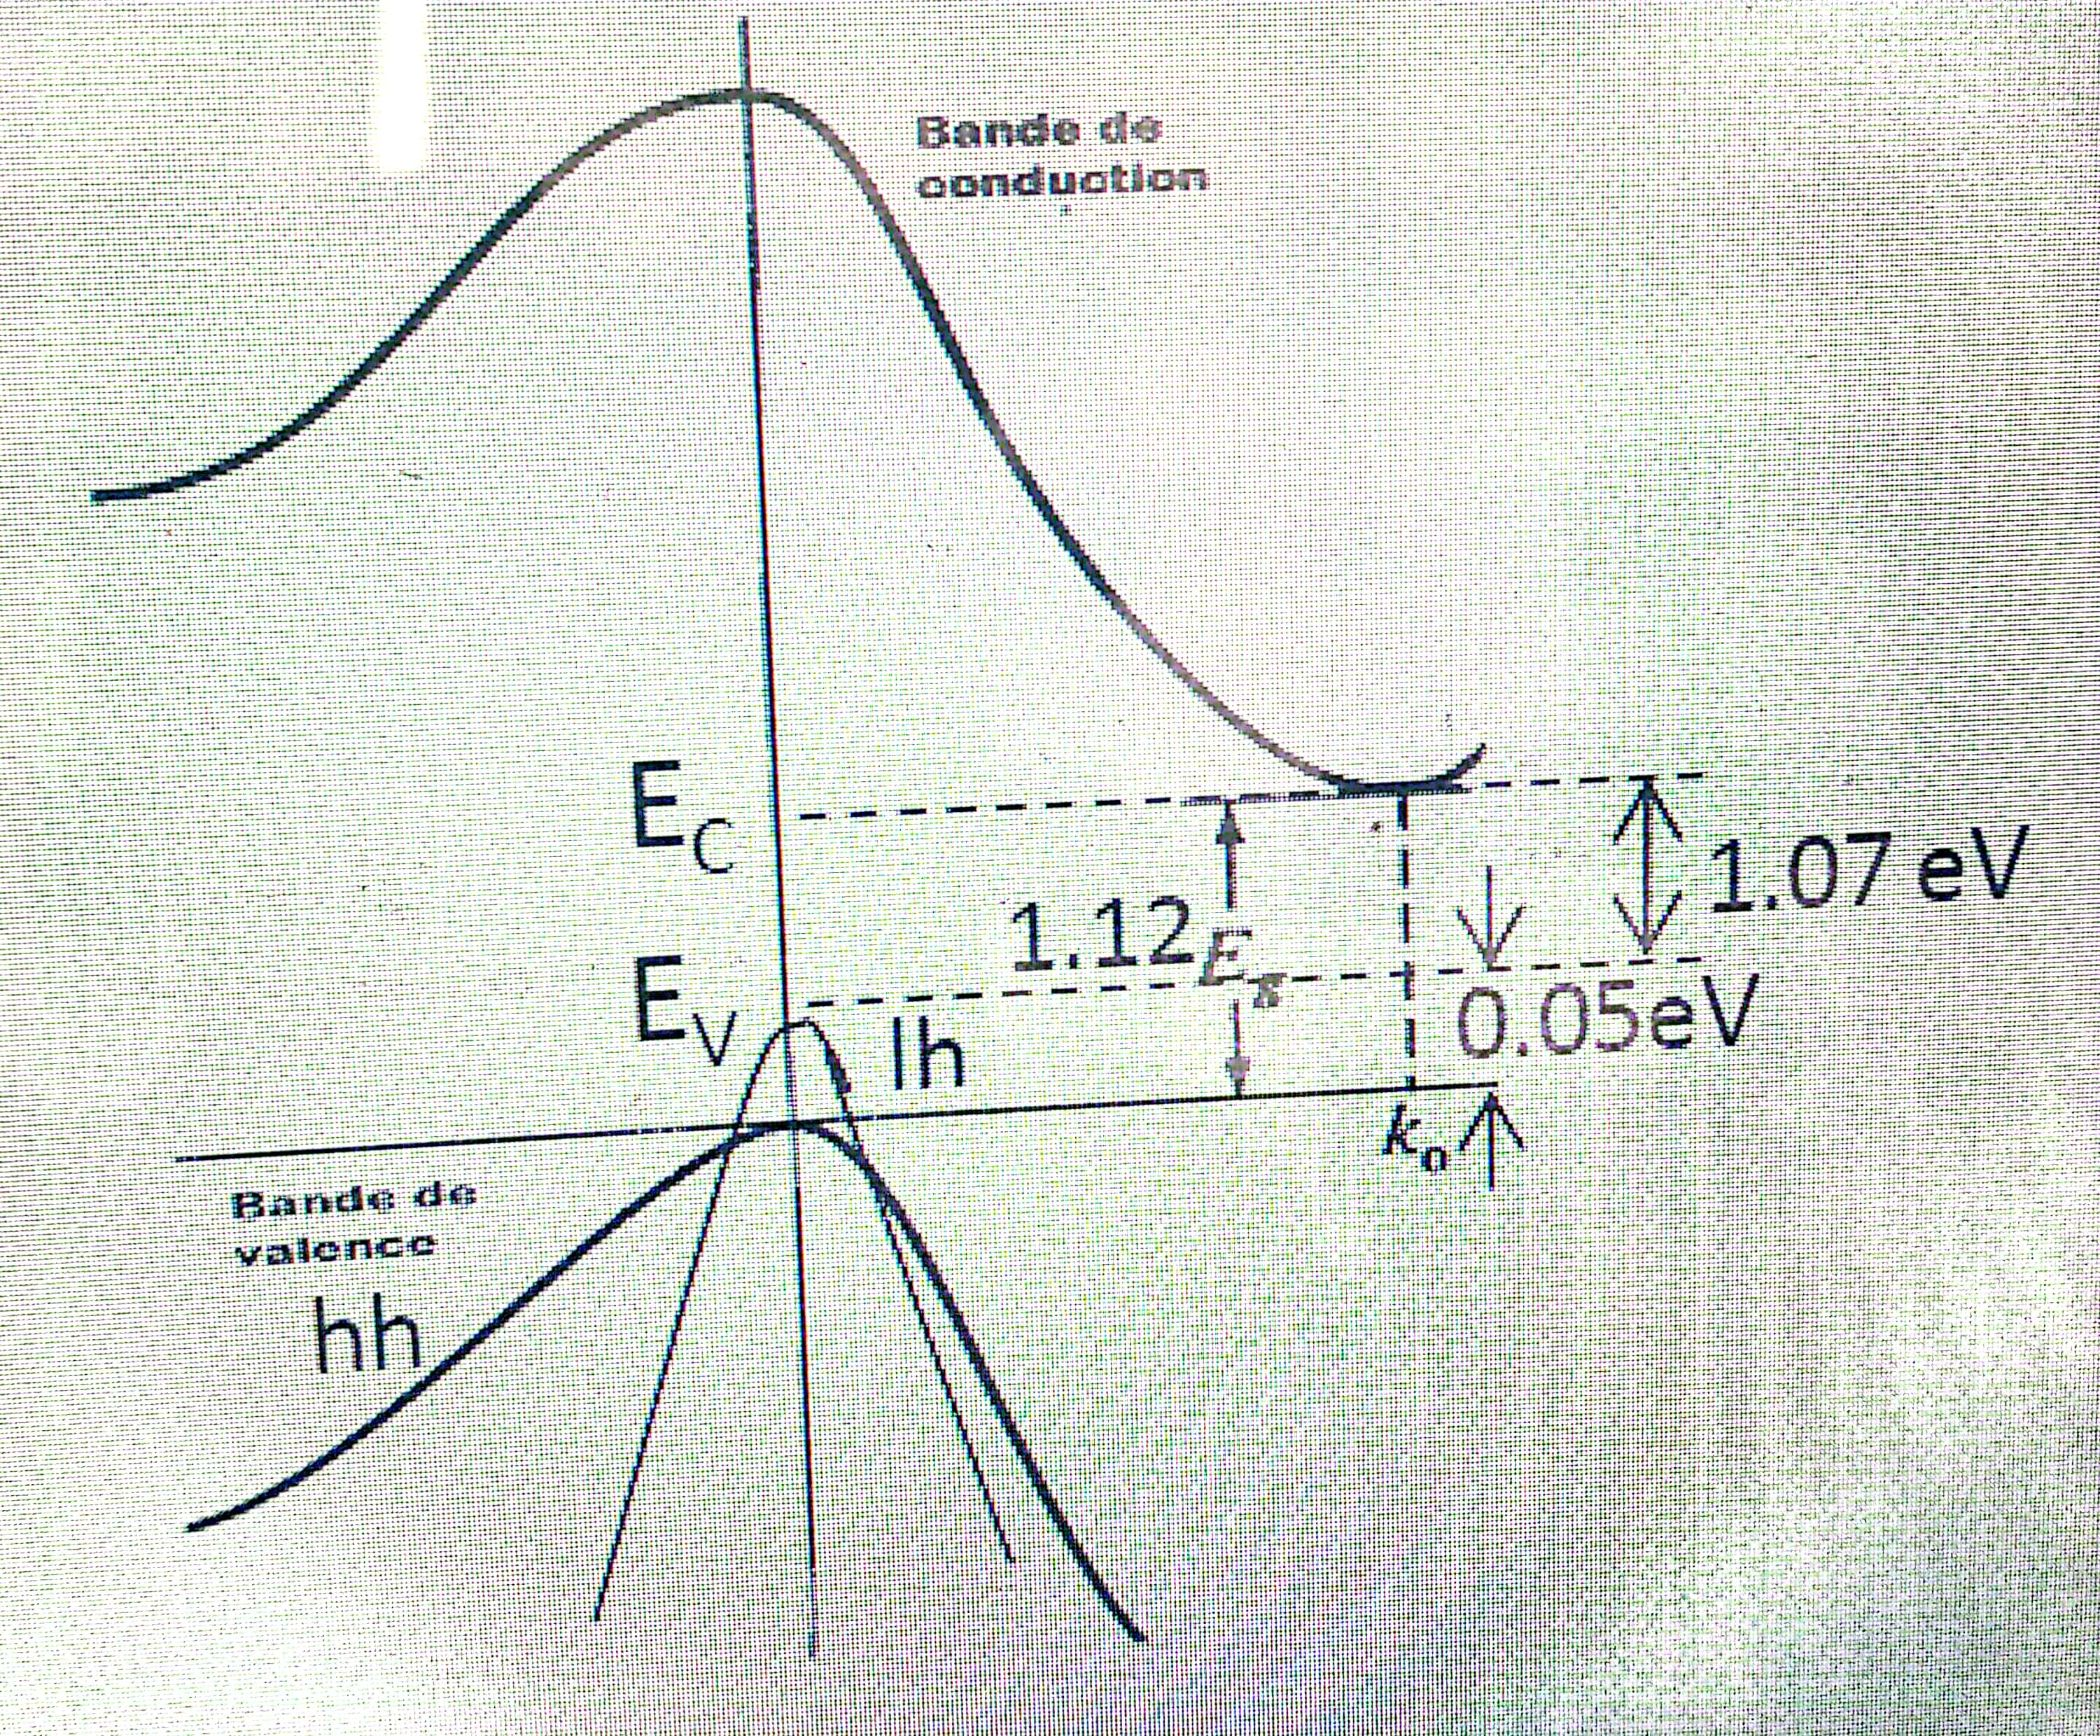
\includegraphics[width=0.55\textwidth]{images/semi_conducteurs/bandes_energie.png}\\[4pt]
{\small\itshape Structure de bandes d'un semi-conducteur : bande de conduction (haut) et bande de valence (bas), séparées par le gap $E_g$.}
\end{center}

\begin{center}
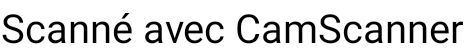
\includegraphics[width=0.6\textwidth]{images/semi_conducteurs/sc-006-000.png}\\[4pt]
{\small\itshape Classification des solides : conducteur, semi-conducteur et isolant selon la largeur du gap.}
\end{center}

\textbf{2.} Classification :
\begin{itemize}[nosep]
  \item Cu : $E_g \approx 0$ $\to$ \textbf{conducteur} (les bandes se chevauchent).
  \item Si : $E_g = \qty{1.12}{eV}$ $\to$ \textbf{semi-conducteur}.
  \item SiO$_2$ : $E_g \approx \qty{9}{eV}$ $\to$ \textbf{isolant}.
\end{itemize}

\textbf{3.} Dans un semi-conducteur, quand $T$ augmente, l'agitation thermique permet à plus d'électrons de franchir le gap, créant davantage de porteurs ($n$ et $p$ augmentent en $\e^{-E_g/2k_BT}$). La conductivité $\sigma = e(n\mu_n + p\mu_p)$ augmente malgré la légère diminution des mobilités. Dans un métal, le nombre de porteurs est constant, et les collisions avec le réseau augmentent, réduisant la mobilité (résistivité croissante).

\textbf{4.} On utilise l'approximation $n_i \propto T^{3/2}\e^{-E_g/(2k_BT)}$ :
\[
\frac{n_i(400)}{n_i(300)} = \left(\frac{400}{300}\right)^{3/2}\times\frac{\e^{-E_g/(2k_B\times400)}}{\e^{-E_g/(2k_B\times300)}}
\]
Le terme $T^{3/2}$ : $(400/300)^{3/2} = (4/3)^{3/2} \approx 1{,}54$.
Le terme exponentiel avec $E_g = 1{,}12\,\text{eV}$, $k_B = 8{,}617\times10^{-5}\,\text{eV/K}$ :
\[
\frac{E_g}{2k_B}\left(\frac{1}{300}-\frac{1}{400}\right) = \frac{1{,}12}{1{,}723\times10^{-4}}\times\frac{100}{120000} \approx 6503\times8{,}33\times10^{-4} \approx 5{,}42
\]
\[
\frac{n_i(400)}{n_i(300)} \approx 1{,}54\times\e^{5{,}42} \approx 1{,}54\times226 \approx \boxed{348}
\]
À 400\,K, $n_i$ est environ 350 fois plus grande qu'à 300\,K.
\end{boitecorrige}

\subsection*{Exercice 7 - Potentiel de contact et zone de déplétion \niveau{\moyen}}

\begin{boiteexercice}
Une jonction abrupte p-n en silicium ($\varepsilon_r = 11{,}7$, $\varepsilon_0 = \qty{8.85e-12}{F.m^{-1}}$) à 300\,K possède : $N_A = \qty{1e17}{cm^{-3}}$ côté p et $N_D = \qty{1e15}{cm^{-3}}$ côté n. On donne $n_i = \qty{1.5e10}{cm^{-3}}$ et $V_T = k_BT/e = \qty{25.85}{mV}$.
\begin{enumerate}
  \item Calculer la tension de contact $V_0$.
  \item La largeur de la zone de déplétion côté n est $x_n = \sqrt{\dfrac{2\varepsilon V_0}{e}\,\dfrac{N_A}{N_D(N_A+N_D)}}$. Calculer $x_n$ et $x_p = x_n N_D/N_A$.
  \item Calculer le champ électrique maximal $E_{max} = eN_Dx_n/\varepsilon$ (en V/cm).
\end{enumerate}
\end{boiteexercice}

\begin{boitecorrige}
\textbf{1.}
\[
V_0 = V_T\ln\!\left(\frac{N_A N_D}{n_i^2}\right) = 0{,}02585\times\ln\!\left(\frac{10^{17}\times10^{15}}{(1{,}5\times10^{10})^2}\right)
\]
\[
= 0{,}02585\times\ln\!\left(\frac{10^{32}}{2{,}25\times10^{20}}\right) = 0{,}02585\times\ln(4{,}44\times10^{11})
\]
\[
= 0{,}02585\times\ln(4{,}44\times10^{11}) = 0{,}02585\times26{,}8 \approx \boxed{\qty{0.693}{V}}
\]

\textbf{2.} Permittivité absolue : $\varepsilon = \varepsilon_r\varepsilon_0 = 11{,}7\times8{,}85\times10^{-12} = \qty{1.036e-10}{F.m^{-1}}$.

\begin{center}
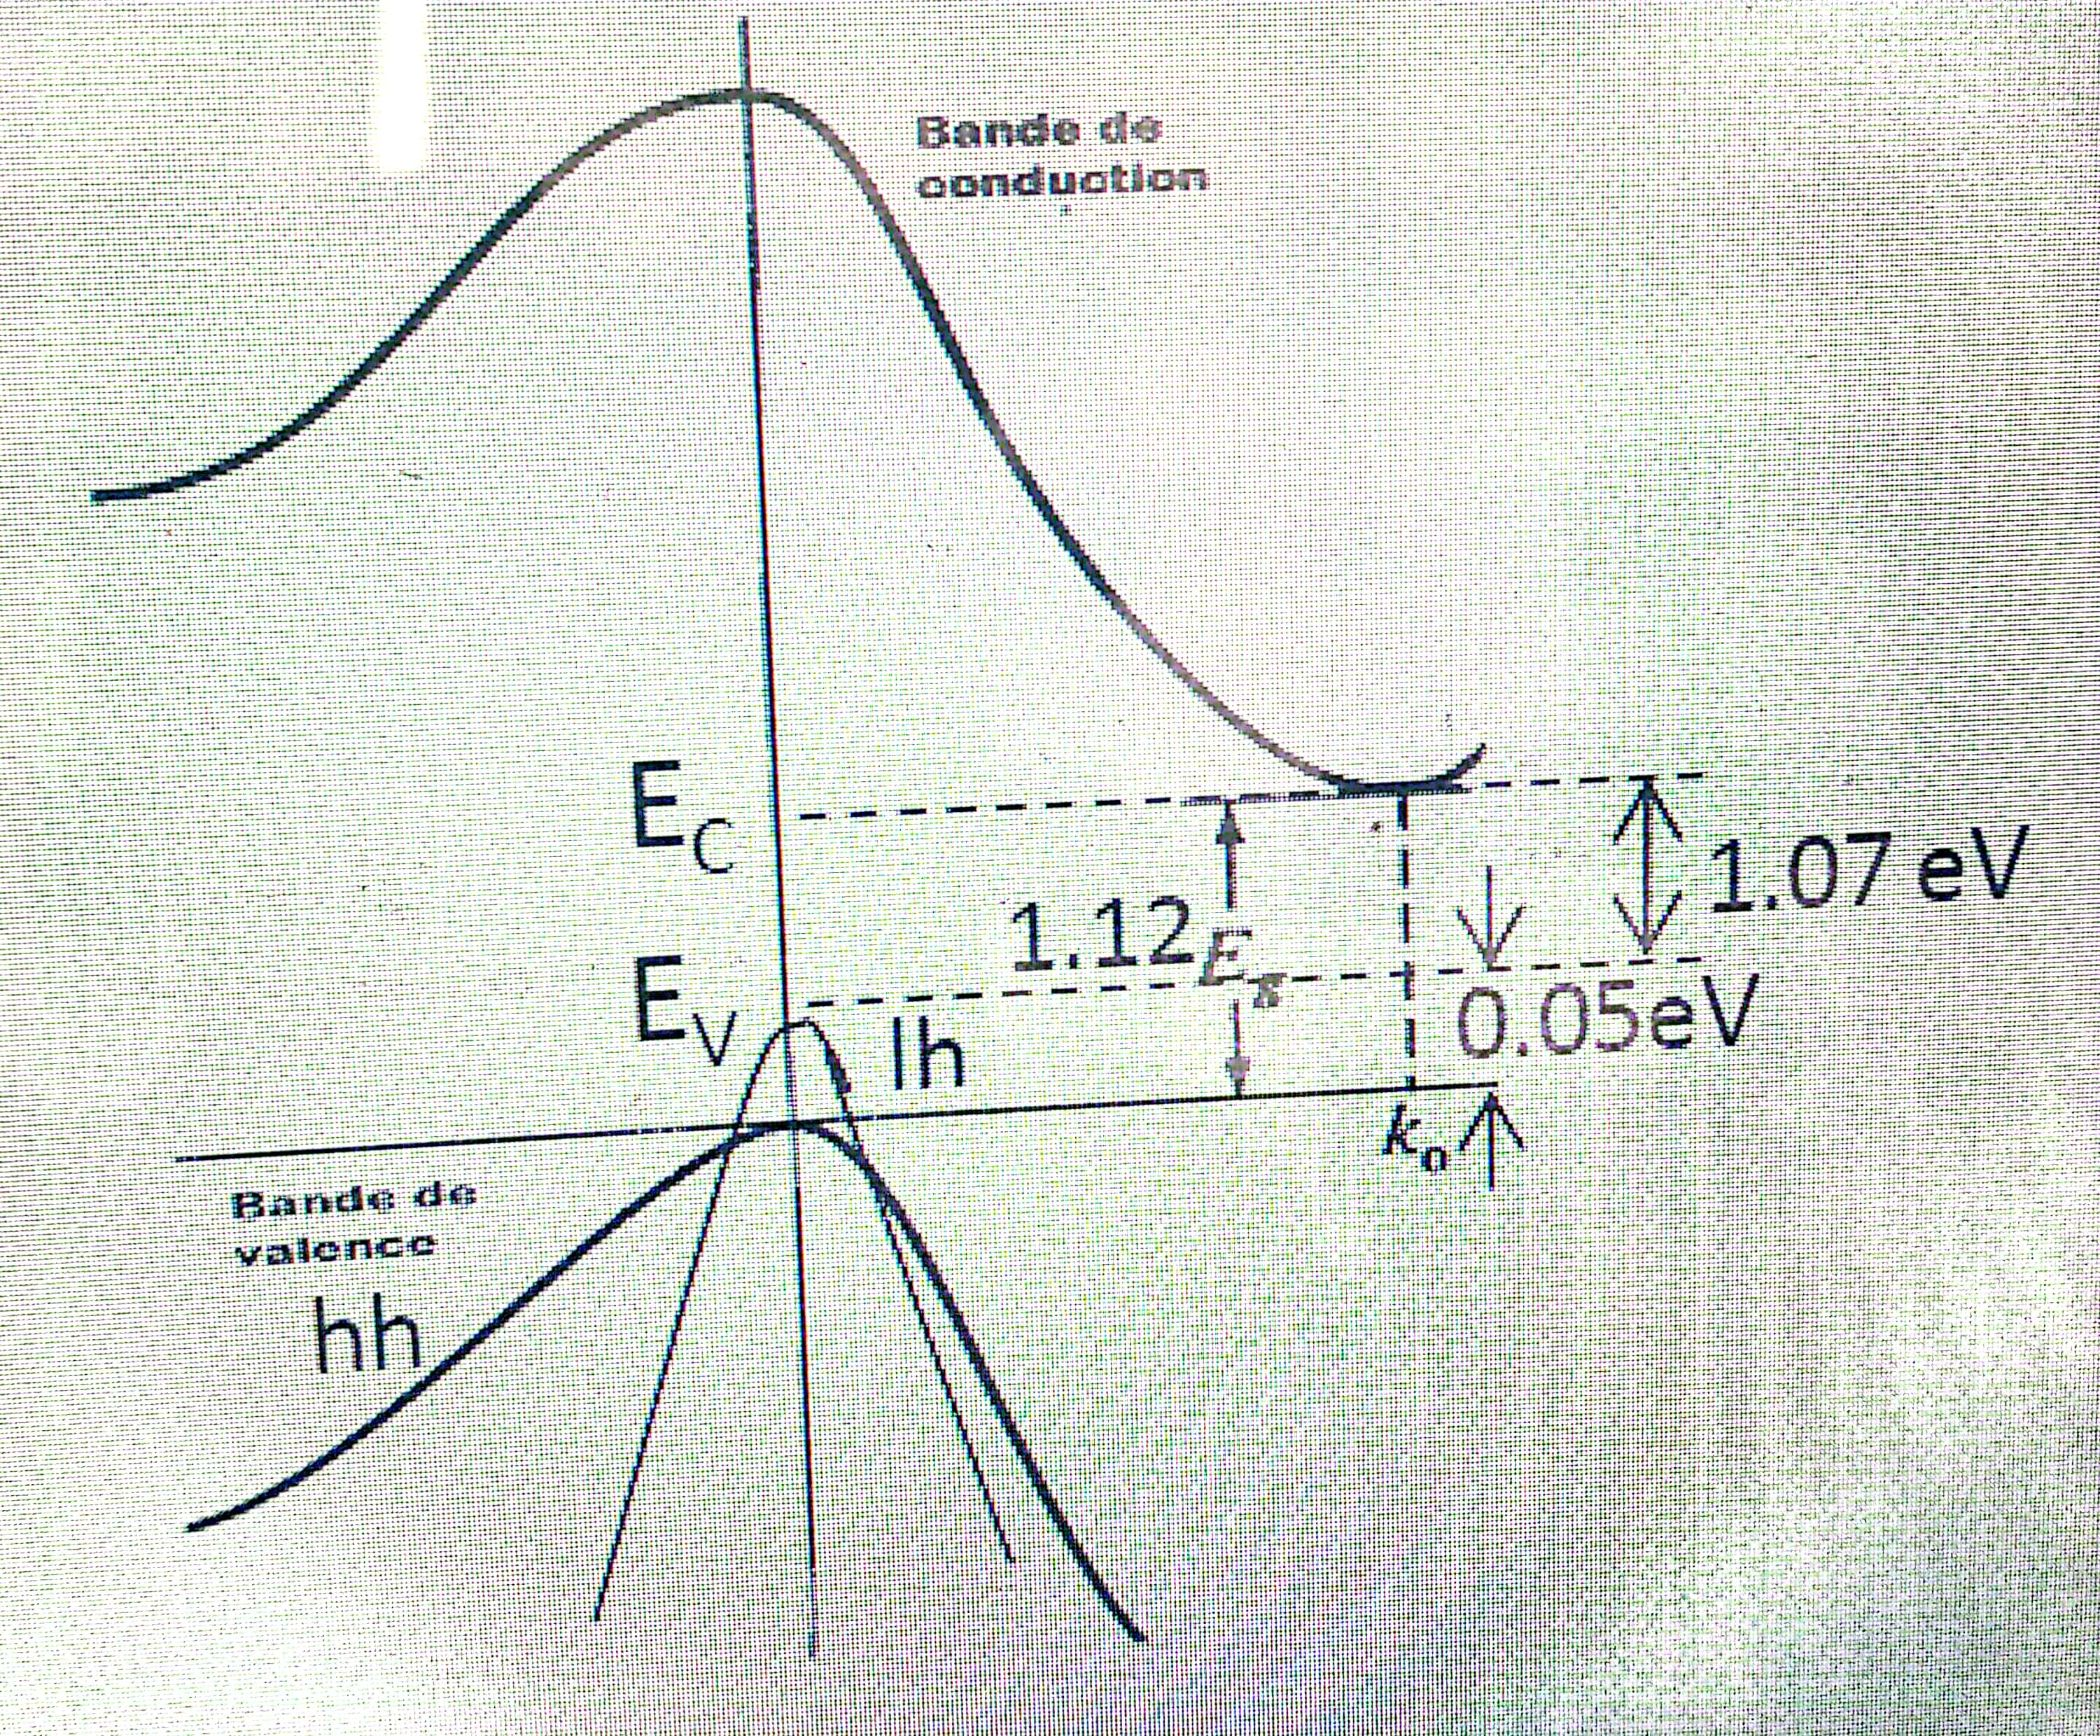
\includegraphics[width=0.7\textwidth]{images/semi_conducteurs/sc-006-001.png}\\[4pt]
{\small\itshape Jonction p-n à l'équilibre : zone de déplétion, champ interne et tension de contact $V_0$.}
\end{center}

Avec $N_D = 10^{15}\,\text{cm}^{-3} = 10^{21}\,\text{m}^{-3}$, $N_A = 10^{17}\,\text{cm}^{-3} = 10^{23}\,\text{m}^{-3}$, $e = \qty{1.6e-19}{C}$ :
\begin{align*}
x_n &= \sqrt{\frac{2\times1{,}036\times10^{-10}\times0{,}693}{1{,}6\times10^{-19}}\,\frac{10^{23}}{10^{21}(10^{23}+10^{21})}}\\
&\approx \sqrt{\frac{1{,}435\times10^{-10}}{1{,}6\times10^{-19}}\,\frac{10^{23}}{1{,}01\times10^{21}\times10^{23}}}\\
&= \sqrt{\frac{1{,}435\times10^{-10}}{1{,}6\times10^{-19}}\times\frac{1}{1{,}01\times10^{21}}}
\approx \sqrt{8{,}87\times10^{-13}} \approx \qty{9.4e-7}{m} = \qty{0.94}{\mu m}
\end{align*}

$x_p = x_n\times N_D/N_A = 0{,}94\times10^{15}/10^{17} = \qty{9.4e-3}{\mu m} = \qty{9.4}{nm}$

\textbf{3.} Champ électrique maximal :
\[
E_{max} = \frac{eN_Dx_n}{\varepsilon} = \frac{1{,}6\times10^{-19}\times10^{21}\times9{,}4\times10^{-7}}{1{,}036\times10^{-10}} \approx \qty{1.45e5}{V.m^{-1}} = \qty{1450}{V.cm^{-1}}
\]
\end{boitecorrige}

\subsection*{Exercice 8 - Équation de Shockley et caractéristique I-V \niveau{\moyen}}

\begin{boiteexercice}
Une diode au silicium à 300\,K a un courant de saturation $I_s = \qty{10}{nA}$ et $V_T = \qty{25.85}{mV}$.
\begin{enumerate}
  \item Rappeler l'équation de Shockley $I = I_s(\e^{V/V_T}-1)$ et ses hypothèses.
  \item Calculer $I$ pour $V = \qty{0.5}{V}$ (direct) et $V = \qty{-5}{V}$ (inverse).
  \item Trouver la tension $V$ telle que $I = \qty{1}{mA}$.
  \item On veut polariser la diode à $I_0 = \qty{5}{mA}$ avec une alimentation $V_{CC} = \qty{5}{V}$. Calculer la résistance de limitation $R$ nécessaire (en supposant $V_D \approx \qty{0.65}{V}$).
\end{enumerate}
\end{boiteexercice}

\begin{boitecorrige}
\textbf{1.} L'équation de Shockley $I = I_s(\e^{V/V_T}-1)$ décrit la caractéristique I-V d'une jonction idéale. Elle repose sur les hypothèses : porteurs minoritaires peu nombreux (faible injection), pas de recombinaison dans la zone de déplétion, jonction abrupte. $V_T = k_BT/e$ est la tension thermique.

\textbf{2.}
\begin{itemize}[nosep]
  \item Polarisation directe $V = \qty{0.5}{V}$ : $\e^{0{,}5/0{,}02585} = \e^{19{,}34} \approx 2{,}50\times10^8$.
  \[
  I = 10\times10^{-9}\times(2{,}50\times10^8 - 1) \approx 10\times10^{-9}\times2{,}50\times10^8 = \qty{2.5}{A}
  \]
  \item Polarisation inverse $V = \qty{-5}{V}$ : $\e^{-5/0{,}02585} = \e^{-193} \approx 0$, donc $I \approx -I_s = \qty{-10}{nA}$.
\end{itemize}

\textbf{3.} Pour $I = \qty{1}{mA}$ :
\[
\e^{V/V_T} = 1 + \frac{I}{I_s} = 1 + \frac{10^{-3}}{10^{-8}} = 10^5
\]
\[
V = V_T\ln(10^5) = 0{,}02585\times5\ln(10) = 0{,}02585\times11{,}51 \approx \boxed{\qty{0.298}{V}}
\]
(En pratique, la tension de seuil réelle du Si est plutôt autour de 0,6--0,7\,V à cause des recombinaisons.)

\textbf{4.} La loi des mailles : $V_{CC} = R\cdot I_0 + V_D$, d'où :
\[
R = \frac{V_{CC} - V_D}{I_0} = \frac{5 - 0{,}65}{5\times10^{-3}} = \frac{4{,}35}{5\times10^{-3}} = \boxed{\qty{870}{\Omega}}
\]
\end{boitecorrige}

\subsection*{Exercice 9 - Transport et mobilité des porteurs \niveau{\moyen}}

\begin{boiteexercice}
Un barreau de silicium de type N ($N_D = \qty{1e16}{cm^{-3}}$, $\mu_n = \qty{1350}{cm^2.V^{-1}.s^{-1}}$, $\mu_p = \qty{480}{cm^2.V^{-1}.s^{-1}}$, $n_i = \qty{1.5e10}{cm^{-3}}$) est soumis à un champ électrique $\vec{E} = \qty{100}{V.cm^{-1}}$.
\begin{enumerate}
  \item Calculer la densité d'électrons $n$ et de trous $p$ à 300\,K.
  \item Calculer la conductivité $\sigma$ et la résistivité $\rho$.
  \item Calculer les vitesses de dérive $v_n = \mu_n E$ et $v_p = \mu_p E$ des électrons et des trous.
  \item Calculer les densités de courant de dérive $J_n = en\mu_n E$ et $J_p = ep\mu_p E$. Quelle est la densité de courant totale ?
\end{enumerate}
\end{boiteexercice}

\begin{boitecorrige}
\textbf{1.} $N_D = \qty{1e16}{cm^{-3}} \gg n_i$ :
\[
n \approx N_D = \qty{1e16}{cm^{-3}} \qquad p = \frac{n_i^2}{n} = \frac{(1{,}5\times10^{10})^2}{10^{16}} = \qty{2.25e4}{cm^{-3}}
\]

\textbf{2.}
\[
\sigma = e(n\mu_n + p\mu_p) \approx en\mu_n = 1{,}6\times10^{-19}\times10^{16}\times1350 = \qty{2.16}{S.cm^{-1}}
\]
\[
\rho = 1/\sigma \approx \qty{0.463}{\Omega.cm}
\]

\textbf{3.} Vitesses de dérive (en valeur absolue) :
\[
v_n = \mu_n E = 1350\times100 = \qty{1.35e5}{cm.s^{-1}} = \qty{1350}{m.s^{-1}}
\]
\[
v_p = \mu_p E = 480\times100 = \qty{4.8e4}{cm.s^{-1}} = \qty{480}{m.s^{-1}}
\]
Les électrons dérivent en sens inverse du champ, les trous dans le sens du champ.

\textbf{4.}
\[
J_n = en\mu_n E = 1{,}6\times10^{-19}\times10^{16}\times1350\times100 = \qty{216}{A.cm^{-2}}
\]
\[
J_p = ep\mu_p E = 1{,}6\times10^{-19}\times2{,}25\times10^4\times480\times100 \approx \qty{1.7e-10}{A.cm^{-2}} \approx 0
\]
\[
J_{total} = J_n + J_p \approx \qty{216}{A.cm^{-2}}
\]
La contribution des trous (porteurs minoritaires) est totalement négligeable.
\end{boitecorrige}

\subsection*{Exercice 10 - Transistor à effet de champ (MOSFET) \niveau{\difficile}}

\begin{boiteexercice}
Un transistor NMOS (canal N) a les paramètres suivants : tension de seuil $V_T = \qty{1}{V}$, transconductance $\mu_n C_{ox} W/L = k = \qty{2}{mA.V^{-2}}$.
\begin{enumerate}
  \item Expliquer le principe de fonctionnement du MOSFET : comment le champ électrique de grille crée-t-il un canal conducteur ?
  \item En régime saturé ($V_{DS} \geq V_{GS} - V_T$), le courant de drain est $I_D = \dfrac{k}{2}(V_{GS}-V_T)^2$. Calculer $I_D$ pour $V_{GS} = \qty{3}{V}$.
  \item En régime linéaire ($V_{DS} < V_{GS}-V_T$), $I_D = k\left[(V_{GS}-V_T)V_{DS} - \dfrac{V_{DS}^2}{2}\right]$. Calculer $I_D$ pour $V_{GS} = \qty{3}{V}$ et $V_{DS} = \qty{0.5}{V}$.
  \item Calculer la résistance du canal $r_{DS} = V_{DS}/I_D$ en régime linéaire avec $V_{DS} \to 0$.
\end{enumerate}
\end{boiteexercice}

\begin{boitecorrige}
\textbf{1.} Dans un MOSFET à canal N, l'application d'une tension positive $V_{GS}$ sur la grille crée un champ électrique qui attire les électrons minoritaires (substrat p) vers l'interface oxyde-silicium. Pour $V_{GS} > V_T$, une couche d'inversion (canal N) se forme entre source et drain. Le courant $I_D$ est contrôlé par $V_{GS}$, d'où l'effet de champ (FET = Field Effect Transistor).

\textbf{2.} Régime saturé avec $V_{GS} = \qty{3}{V}$, $V_T = \qty{1}{V}$ :
\[
I_D = \frac{k}{2}(V_{GS}-V_T)^2
   = \frac{2\times10^{-3}}{2}(3-1)^2
   = 10^{-3}\times4 = \qty{4}{mA}
\]

\textbf{3.} Régime linéaire avec $V_{GS} = \qty{3}{V}$, $V_{DS} = \qty{0.5}{V}$ (vérifions : $V_{DS} = 0{,}5 < V_{GS}-V_T = 2$ : oui, régime linéaire) :
\begin{align*}
I_D &= 2\times10^{-3}\times\left[(3-1)\times0{,}5 - \frac{(0{,}5)^2}{2}\right]\\
    &= 2\times10^{-3}\times(1 - 0{,}125)\\
    &= 2\times10^{-3}\times0{,}875 = \qty{1.75}{mA}
\end{align*}

\textbf{4.} En régime linéaire pour $V_{DS} \ll V_{GS}-V_T$ :
\[
I_D \approx k(V_{GS}-V_T)V_{DS} \quad\Rightarrow\quad r_{DS} = \frac{V_{DS}}{I_D} = \frac{1}{k(V_{GS}-V_T)} = \frac{1}{2\times10^{-3}\times2} = \qty{250}{\ohm}
\]
Plus $V_{GS}$ est élevé, plus le canal est ouvert (résistance faible).
\end{boitecorrige}

\ifdefined\inMainDoc\else\end{document}\fi
